% !Mode:: "TeX:UTF-8"
\documentclass[landt]{skythesis}
\graphicspath{{figures/}}  % 图路径
%% 文献翻译和原文需要的链接
\newcommand{\kappendix}[2][section]{
 \phantomsection
 \addcontentsline{toc}{#1}{#2}
}

\begin{document}
% !Mode:: "TeX:UTF-8"
%% 封面
%% 信息填写
%论文题目:{中文}
\skytitle{论文题目是论文的题目}
%论文英文题目:
\Skytitle{Paper's Title is Paper's Tilte}
%作者:{中文姓名}{学号}
\skyauthor{我是作者}{00000000}
%拼音
\Skyauthor{I am the fucking author}
%指导教师:{导师中文名}
\skymentor{我是导师}
%拼音
\Skymentor{I am your mentor}
%个人信息:{毕业年份}{专业}
\skyinfo{2014}{我是专业}
%班级
\skyclass{我是班级}
%学院信息:{学院中文}
\skycollege{我是学院}
%英文信息
\Skycollege{I'm college name}
%学校名称:
\skyschool{浙江工业大学}
%英文校名
\Skyschool{Zhejiang University of Technology}
\thispagestyle{empty}
\pdfbookmark[-1]{封~~面}{thesiscover}
\phantomsection \label{thesiscover} %无形节命令
\newcommand\midtitle{}

\ifskythesis
  \renewcommand\midtitle{毕业论文(毕业设计说明书)}
\fi
\ifskylandt
  \renewcommand\midtitle{毕业论文(文献综述、外文翻译)}
\fi
\ifskyproposal
  \renewcommand\midtitle{毕业论文(开题报告)}
\fi
\vspace*{10mm}
% 校名
\begin{center}
   
\includegraphics[height=42pt,trim= 0 300 0 0]{zjutlogo}{\stxingkai\juhao{~浙江工业大学}}
\end{center}
\vspace*{12mm}
\centerline{\linespread{1.5}\songti\yihao\bf\midtitle}
\vspace*{19mm}

\renewcommand{\arraystretch}{1.0} %列表行距
\hspace*{3mm} 

{\sfzhongsong\yihao{题目}
\hspace{0mm} 
\begin{minipage}[t]{120mm} % 这里建议自行微调
 \centering 
 \renewcommand{\ULthickness}{1.2pt}
 \renewcommand{\CJKunderlinecolor}{\color{black}}
   \linespread{1.1}\CJKunderline{\quad\skytitlec\quad}
\end{minipage}
}

\vspace*{15mm}
\begin{center}
    %\setlength{\arrayrulewidth}{0.5pt}
    
    {\sfzhongsong\sanhao
    \renewcommand{\ULthickness}{1.2pt}
    \renewcommand{\CJKunderlinecolor}{\color{black}}
    \newcommand{\kdist}{\hspace{4em}}
    
        \renewcommand{\arraystretch}{1.5}
        \begin{tabular}{lc}
            专\hspace{2em}业:& \CJKunderline{\kdist\extt{\skymajor}\kdist} \\ 
            班\hspace{2em}级: & \CJKunderline{\kdist\extt{\skyclassc}\kdist} \\
            学生姓名: &  \CJKunderline{\kdist\extt{\skyauthornamec}\kdist}\\
            指导老师: & \CJKunderline{\kdist\extt{\skymentorc}\kdist} \\
        \end{tabular}
    }
\vspace{60mm}

{\sfzhongsong\sihao 2013-2014学年}
\end{center}

      % 封面

\frontmatter
%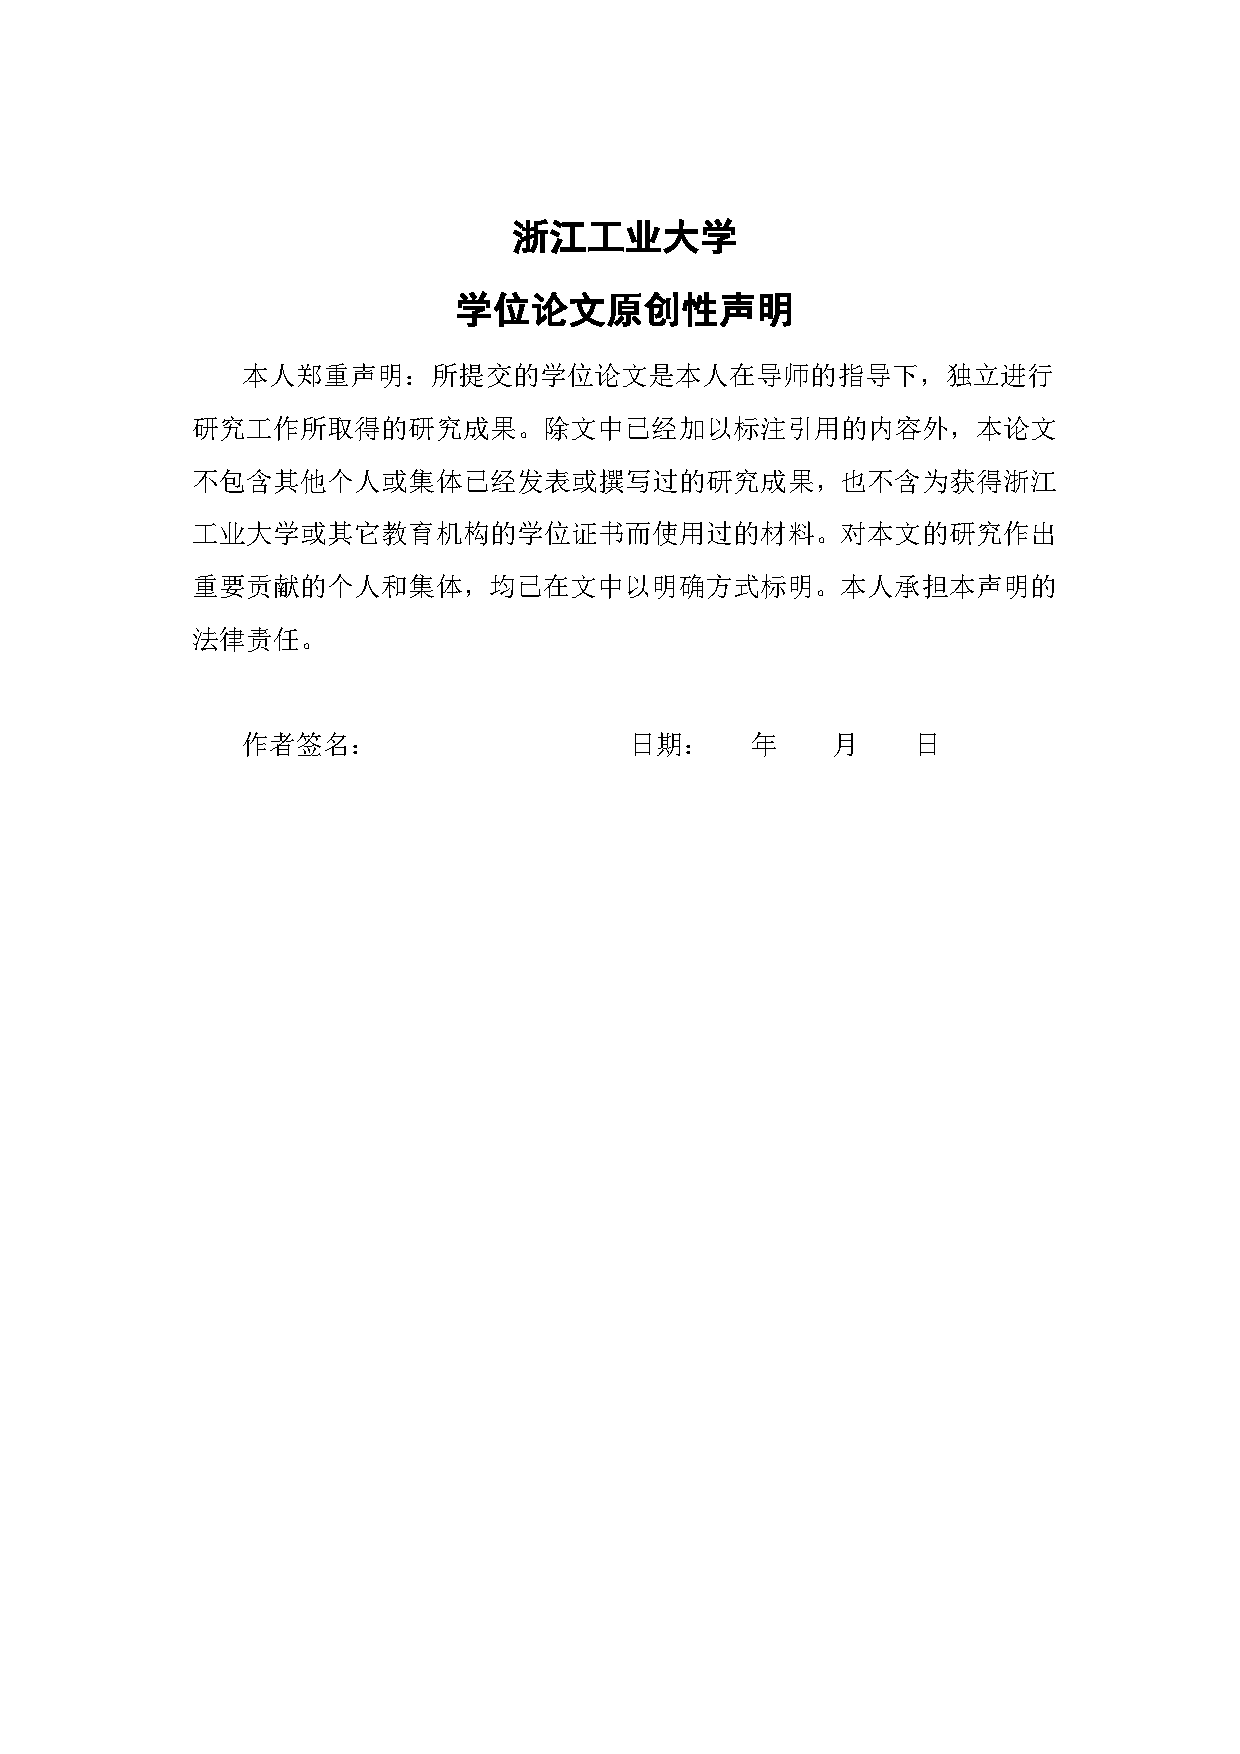
\includepdf{preface/statement}
\pagenumbering{Roman}

%% !Mode:: "TeX:UTF-8"
%% 中文摘要
\begin{abstractc}
\begin{center}
{
\xiaosi
\vspace{1em}

 学生姓名:\skyauthornamec \hspace{20mm} 指导老师:\skymentorc

\skyschoolc\skycollegec}

{\xiaosan\bf\vbox{} \heiti {摘\quad 要}}
\vspace{-1cm}
\end{center}

{\sihao \songti \indent

\input{preface/mainc.txt}
}
\end{abstractc}     % 中文摘要
%% !Mode:: "TeX:UTF-8"
%% 英文摘要
\begin{abstracte}
\begin{center}
\vspace{1em}
{\xiaosi \onehalfspacing
 Author: \Skyauthorc\hspace{20mm} Mentor: \Skymentorc

\Skycollegec, \Skyschoolc

{\xiaosan\bf\vbox{} Abstract}
}
\end{center}

{
\indent \sihao \input{preface/maine.txt}}
\end{abstracte}
     % English Abstract
{\pdfbookmark[0]{目~~录}{thiscontent}\phantomsection \label{thiscontent}\singlespacing\tableofcontents           % 中文目录
}

%%%%%%%%%% 正文 %%%%%%%%%%
\mainmatter
\makeatletter
% !Mode:: "TeX:UTF-8"
%%  绪论
\chapter{绪论}
\section{课题研究的背景和意义}

\section{课题研究的国内外现状}



% !Mode:: "TeX-UTF-8"
\chapter{***相关理论}
% !Mode:: "TeX:UTF-8"
\chapter{案例分析}


% !Mode:: "TeX:UTF-8"
\chapter{总结}


\makeatother
\backmatter

%%%%%%%%%% 参考文献 %%%%%%%%%%
\bibliography{references/reference}
\nocite{*}   % 若将此命令屏蔽掉,则未引用的文献不会出现在文后的参考文献中。

%%%%%%%%%% 附录 %%%%%%%%%%
% !Mode:: "TeX:UTF-8"
%% 文献翻译中使用的标题
\newcommand\kchapter[1]{\stepcounter{chapter}\chapter*{\the\value{chapter}#1}}
\newcommand\ksection[1]{\stepcounter{section}\section*{\the\value{chapter}.\the\value{section}#1}}
\newcommand\ksubsection[1]{\stepcounter{subsection}\subsection*{\the\value{chapter}.\the\value{section}.\the\value{subsection}#1}}

%%文献翻译中需要的计数器
\newcounter{app}
\renewcommand{\theapp}{\Alph{app}}
\renewcommand{\thefigure}{\theapp-\arabic{figure}}
\renewcommand{\thetable}{\theapp-\arabic{table}}
\renewcommand{\theequation}{\theapp.\arabic{equation}}

%% 文献翻译环境
\newpage
\begin{transcript}
	\kappendix[chapter]{文献翻译}
	% !Mode:: "TeX:UTF-8"
\stepcounter{app}
\begin{Abstract}
\chapter*{文献翻译示例}\addcontentsline{toc}{section}{文献翻译示例}
\begin{center}
\vspace{2mm}
{
 {\xiaosi here you can put the author of the original literature}

 {\xiaowu and his/her address}
}
\end{center}
{\wuhao \songti 
\noindent \textbf{摘要:}我是文献翻译的摘要

\keywords{那我就是关键词了}
}
\end{Abstract}

\kchapter{引言}
然后就开始各章节吧!
%% !Mode:: "TeX:UTF-8"
\kchapter{现行调度方法}
下面将引入相关符号,并对案例中的工厂所运用的现行调度方法进行描述。
\ksection{符合说明与相关假设}
为了方便问题描述,符号说明如下:
\ksection{生产制造过程}

\ksection{准备时间和产品簇}

\ksection{目标函数}

\ksection{现行调度方法}
%% !Mode:: "TeX:UTF-8"
\kchapter{方法改进}

\ksection{456}
%% !Mode:: "TeX:UTF-8"
\kchapter{方法改进}

\ksection{456}
\kchapter{总结和展望}
  %% 接着input 即可

\end{transcript}
\clearpage            % 文献翻译
% !Mode:: "TeX:UTF-8"
\newpage
\includepdfset{pagecommand={\thispagestyle{plain}}}
\kappendix[chapter]{文献原文}
\kappendix{a case study}
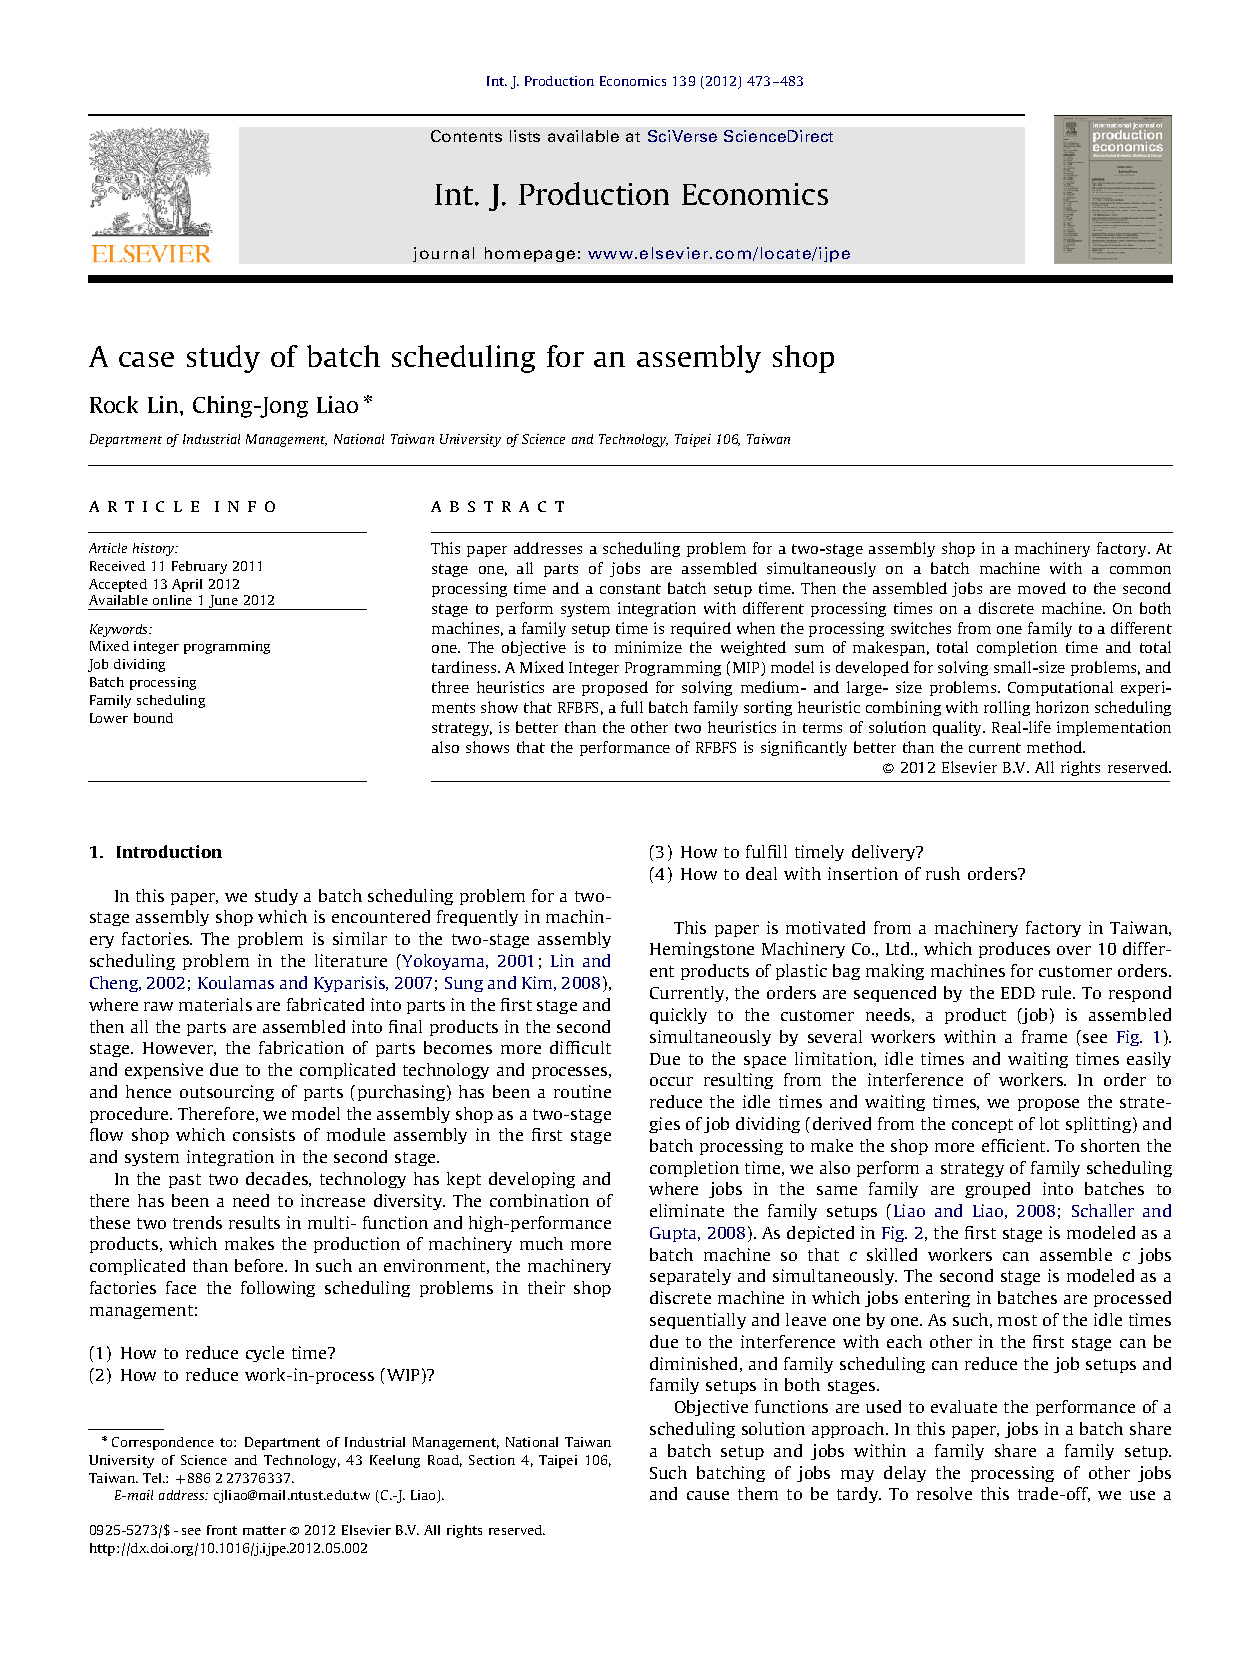
\includepdf[pages=1]{literature/a.pdf}          % 文献原文

\end{document}                                  % 结束全文
